% --------------------------------------------------------------
% This is all preamble stuff that you don't have to worry about.
% Head down to where it says "Start here"
% --------------------------------------------------------------
 
\documentclass[12pt]{article}
\usepackage{graphicx}
\graphicspath{ {./Images/} }
\usepackage[margin=1in]{geometry} 
\usepackage{amsmath,amsthm,amssymb}
\usepackage[margin=1in]{geometry} 
\usepackage{amsmath,amsthm,amssymb}
% \usepackage[spanish]{babel} %Castellanización
\usepackage{tabularx}
\usepackage[T1]{fontenc} %escribe lo del teclado
\usepackage[utf8]{inputenc} %Reconoce algunos símbolos
\usepackage{lmodern} %optimiza algunas fuentes
\usepackage{graphicx}
\graphicspath{ {images/} }
\usepackage{hyperref} % Uso de links
\usepackage{cite}
\usepackage{ifthen}
\usepackage{tikz-qtree}
\usepackage{float}
\usepackage{pgfplots}
\floatstyle{plaintop}
\restylefloat{table}
\usepackage[tableposition=top]{caption}
\usepackage{varwidth}
 \geometry{
 a4paper,
 total={170mm,257mm},
 left=20mm,
 top=15mm,
 bottom=19mm,
 }
 
 \usepackage{siunitx}
\sisetup{per=slash, load=abbr}

    % GRAPHICS
\usepackage{tikz}
\usepackage{pgfplots}
\pgfplotsset{width=7cm,compat=1.3}

 
 
\newcommand{\N}{\mathbb{N}}
\newcommand{\Z}{\mathbb{Z}}
 
\newenvironment{theorem}[2][Theorem]{\begin{trivlist}
\item[\hskip \labelsep {\bfseries #1}\hskip \labelsep {\bfseries #2.}]}{\end{trivlist}}
\newenvironment{lemma}[2][Lemma]{\begin{trivlist}
\item[\hskip \labelsep {\bfseries #1}\hskip \labelsep {\bfseries #2.}]}{\end{trivlist}}
\newenvironment{exercise}[2][Exercise]{\begin{trivlist}
\item[\hskip \labelsep {\bfseries #1}\hskip \labelsep {\bfseries #2.}]}{\end{trivlist}}
\newenvironment{problem}[2][Problem]{\begin{trivlist}
\item[\hskip \labelsep {\bfseries #1}\hskip \labelsep {\bfseries #2.}]}{\end{trivlist}}
\newenvironment{question}[2][Question]{\begin{trivlist}
\item[\hskip \labelsep {\bfseries #1}\hskip \labelsep {\bfseries #2.}]}{\end{trivlist}}
\newenvironment{corollary}[2][Corollary]{\begin{trivlist}
\item[\hskip \labelsep {\bfseries #1}\hskip \labelsep {\bfseries #2.}]}{\end{trivlist}}

\newenvironment{solution}{\begin{proof}[Solution]}{\end{proof}}

%quiggly arrow things
\newcommand{\squig}{$\scriptsize$\sim$\normalsize$\!}
\newcommand{\lsquigend}{$\scriptsize$\lhd\!$\normalsize$}
\newcommand{\rsquigend}{$\scriptsize\rule{.1ex}{0ex}$\rhd$\normalsize$}


\newcounter{index}

\newcommand\squigs[1]{%
  \setcounter{index}{0}%
  \whiledo {\value{index}< #1}
  {\addtocounter{index}{1}\squig}
}

\newcommand\rsquigarrow[2]{$
  \setbox0\hbox{$\squigs{#2}\rsquigend$}%
  \tiny$%
  \!\!\!\!\begin{array}{c}%
  \mathrm{#1}\\%
  \usebox0%
  \end{array}%
  $\normalsize$\!\!%
}

\newcommand\lsquigarrow[2]{$
  \setbox0\hbox{$\lsquigend\squigs{#2}$}%
  \tiny$%
  \!\!\!\!\begin{array}{c}%
  \mathrm{#1}\\%
  \usebox0%
  \end{array}%
  $\normalsize$\!\!%
}
 
 
 
\usepackage{listings}
\usepackage{xcolor}
 
\definecolor{codegreen}{rgb}{0,0.6,0}
\definecolor{codegray}{rgb}{0.5,0.5,0.5}
\definecolor{codepurple}{rgb}{0.58,0,0.82}
\definecolor{backcolour}{rgb}{0.95,0.95,0.92}
 
\lstdefinestyle{mystyle}{
    backgroundcolor=\color{backcolour},   
    commentstyle=\color{codegreen},
    keywordstyle=\color{magenta},
    numberstyle=\tiny\color{codegray},
    stringstyle=\color{codepurple},
    basicstyle=\ttfamily\footnotesize,
    breakatwhitespace=false,         
    breaklines=true,                 
    captionpos=b,                    
    keepspaces=true,                 
    numbers=left,                    
    numbersep=5pt,                  
    showspaces=false,                
    showstringspaces=false,
    showtabs=false,                  
    tabsize=2
}
 
\lstset{style=mystyle}
 

\begin{document}

 
% --------------------------------------------------------------
%                         Start here
% --------------------------------------------------------------

\begin{titlepage} % Suppresses displaying the page number on the title page and the subsequent page counts as page 1
	\newcommand{\HRule}{\rule{\linewidth}{0.5mm}} % Defines a new command for horizontal lines, change thickness here
	
	\center % Centre everything on the page
	
	%------------------------------------------------
	%	Headings
	%------------------------------------------------
	
	\textsc{\LARGE University of Western Australia}\\[1.5cm] % Main heading such as the name of your university/college
	
% 	\textsc{\Large CITS3402}\\[0.5cm] % Major heading such as course name
	
	\textsc{\large High Performance Computing}\\[0.5cm] % Minor heading such as course title
	
	%------------------------------------------------
	%	Title
	%------------------------------------------------
	
	\HRule\\[0.4cm]
	
	{\huge\bfseries Report}\\[0.4cm] % Title of your document
	
	\HRule\\[1.5cm]
	
	%------------------------------------------------
	%	Author(s)
	%------------------------------------------------
	
	\begin{minipage}{0.4\textwidth}
		\begin{flushleft}
			\large
			\textit{Author}\\
			David \textsc{Adams} % Author's name
		\end{flushleft}
	\end{minipage}
	~

	

\vspace{18 mm}
%	\vfill % Position the date 3/4 down the remaining page
	
	{\large\today} % Date, change the \today to a set date if you want to be precise
	
	%------------------------------------------------
	%	Logo
	%------------------------------------------------
% 	  \vfill\vfill  
	  \begin{figure}[h]
	      \centering
	      \includegraphics{tamagotchi_hive.png}
	      \caption{Sourced from XKCD\cite{xkcd}}
	      \label{fig:my_label}
	  \end{figure}
% 	  \includegraphics{Images/seashell.png}
% 	  \caption{Hello world}
	

	 
	%----------------------------------------------------------------------------------------
	
% 	\vfill % Push the date up 1/4 of the remaining page
	
\end{titlepage}

\tableofcontents
\newpage

\section{Introduction}

A shortest path in a graph $G=(V,E)$ is any path $p$ where its weight is equal to that of the minimum weight between two nodes:
\begin{figure}[h]
    \centering

    \[
\delta (u,v) = \begin{cases} min\{w(p): \mbox{ } _u \rsquigarrow{p}{3} _v \}, & \mbox{if there is a path from } u\mbox{ to }v \\
\infty, & \mbox{otherwise } \end{cases}
\]
    \caption{From CLRS \cite{Cormen:2009:IAT:1614191}}
    \label{fig:my_label}
\end{figure}
\\
Computing a shortest path is simple and can be achieved by expanding the lowest weight edge in a sub graph with the root as one node, until all nodes have been reached. This gives the shortest path from a source node to every other node and is known as Dijkstra's algorithm. This process can be repeated for every possible source node in the graph to give the shortest path from any node to any other and is otherwise known as the all pairs shortest path problem. This report examines a way of using Message Passing Interface (MPI) \cite{Forum:1994:MMI:898758} for improving the performance of computing all pairs shortest path.

\subsection{Floyd-Warshall algorithm}

The Floyd-Warshall algorithm is a dynamic programming solution to the all pairs shortest path problem on a directed graph and offers some significant advantages to all pairs Dijkstra in a parallel envrionment.

\subsubsection{Shortest path interpretation}

Floyd-Warshall differs from Dijkstra's algorithm in that it considers paths through intermediate vertices as opposed to the lowest wight edge available. Assuming the vertices of a graph $G$ are $V = \{1,2,\dots, n\}$: \\\\
take \(S=(1,2\dots,k) \subseteq V\) for any two vertices \(i,j \in V\), look at all paths consisting only of nodes from $S$ and consider a shortest path $p$ and a vertex $k$:
\begin{itemize}
    \item if $k$ is an edge vertex of the path (i.e the last node before reaching j from i)
    $p$ it means a path will all the vertices \(\{1,2\dots,k-1\}\) also from a shortest path from i to j
    \item if $k$ is not an edge vertex then the shortest path from i to k will only contain nodes from \(\{1,2\dots,k-1\}\) as k will be a edge node of that path and it is exactly the same for the path k to j \cite{Cormen:2009:IAT:1614191}
\end{itemize}
Because of these observations it is possible to recursively define what a shortest path is slightly differently to how it is in Dijkstra's algorithm. 
\\
Let \(\partial^k_{ij}\) be the weight of a shortest path from i to j through vertices in the set \(S = \{1,2 \dots, k\}\). 
\[
\partial^k_{ij} = \begin{cases} weight[i][j] & \mbox{if } k=0 \\
min(\partial^{k-1}_{ij}, \partial^{k-1}_{ik} + \partial^{k-1}_{kj}) & \mbox{if } k \geq 1 \end{cases}
\]
The reason why the case $k=0$ gives the distance matrix is all the shortest paths through no intermediate nodes at all will just be the weight of the edge from i to j, which is simply whatever the value of the adjacency matrix is for those two nodes. Otherwise the simple question of, 'is the path weight reduced by going through the node k or not'? 
\subsubsection{Pseudo code}

Assuming an adjacency matrix representation where $dist[i][j]$ is the weight of the edge from $i$ to $j$ a simple implementation for the Floyd-warshall algorithm is as follows:

\begin{lstlisting}[language=c, caption=Distributed example]
    for k in vertices:
        for j in vertices:
            for i in vertices:
                if(dist[i][k] + dist[k][j] < dist[i][j] 
                    dist[i][j] = dist[i][k] + dist[i][j]
\end{lstlisting}

\subsubsection{Advantages}

Looking at the Pseudo code it is trivial to derive the complexity of Floyd Warshall of \(\Theta (V^3)\) as for every pair of nodes i and j every intermediate node k is tested to see if it can reduce the current path length. Compared to All pairs Dijkstra's which has an overall complexity of \(\Theta (VElog(V)\) which in the worse case can blow out to \(\Theta (V^3log(V)\) \cite{Cormen:2009:IAT:1614191} for a completely connected graph. There are potentially cases where Dijkstra's can be more optimal, however given an adjacency matrix representation of a graph, Floyd Warshall lend itself much more easily to collective communication and partitioning of the data as well as having the advantage of being able to handle negative edge weight cycles. 

\subsection{Parallelism}
Programs can decrease execution time by running computations in parallel. conceptually, this allows a program to run arbitrary tasks at the same time. Concurrency simulates parallelism and is used to run programs in such a way that it gives the illusion of parallelism. This, however does not provide any execution time benefits. 
\\\\
Parallelism can be implemented differently depending on the use case. The most general software based type of parallelism is known as multiple instruction multiple data (MIMD) parallelism. MIMD allows processors of the parallel system to run asynchronously and independently on separate data.  
\\\\
Note that some tasks are inherently sequential, and thus cannot benefit from parallelism. The main culprit is logical dependency of later instructions on prior parts of the program.
\\\\
Parallel programs must be designed around the type of parallelism implemented. For this project the Message Passing Interface (MPI) is used to achieve MIMD parallelism on a cluster.


\section{Distributed Implementation}
The implemented Floyd-Warshall algorithm splits the input adjacency matrix into groups of rows and equally distributes them to the processors within a cluster. This implementation will be referenced as the row implementation.
\\\\ 
A problem with the row implementation is that it would struggle as the number of vertices become excessively large due to the rows of the matrix becoming increasingly large. This would make rows difficult to store and distribute between processors. an alternative implementation could distribute the matrix as equally sized blocks instead of by rows. This would solve the problem but also increase message sending complexity as more than one processor would have to broadcast to all other processors. This could take advantage of asynchronous communication but would drastically increase code complexity.
\\\\
The row implementation was the final choice for this project due to the graph sizes tested not being excessively large and due to the relatively lower code complexity than that of the alternative implementation.

\subsection{Assumptions}
A few assumptions were made with the given implementation. These are as follows:
\begin{itemize}
    \item All input files are valid
    \item All Processors in the cluster are homogeneous
    \item An input file may be too large for a single processor to store efficiently
    \item No fault tolerance is necessary
    \item There are no negative edge weight cycles
\end{itemize}

\subsection{Data Partitioning}
\label{sec:data}
The data supplied for the program represents an adjacency matrix of a graph and is represented as contiguous integers in a binary file. The file first begins with the number of vertices within the graph followed by The adjacency matrix, that has been flattened into 1 dimension in row major order.
\\\\
To adhere to the assumption that an input may be given that is too large for any single processor to store locally in RAM, it is not feasible to assume that the head processor can read and distribute the whole matrix. Instead, each processor reads an equal amount of rows unless it is not possible to split rows evenly across processors, in which case the first few processors will store one extra row. This provides load balancing in a homogeneous cluster. 
\\\\ 
If the cluster was heterogeneous, each processor could possibly be assigned an efficiency coefficient. This coefficient could alter how the rows are distributed to a given processor to provide heterogeneous load balancing.


\subsection{Process Partitioning}
Each processor is given a subset of vertices from the input graph as explained in section \ref{sec:data} and is responsible for computing the shortest path from the locally stored vertices to all other vertices in the graph. 
\\\\
Distributing the Floyd-Warshall algorithm exploits the fact that each processor holds the distance from its local vertices to all other vertices, and that the algorithm only requires the intermediate vertex k to be retrieved from other processors.
\\\\
To achieve this, each vertex k is broadcasted from the processor it is stored locally to all other processors. The vertex k is then used in each processor to simultaneously run the Floyd-Warshall algorithm on all locally stored processors.

\subsection{Pseudo code}
\label{sec:dist_code}

\begin{lstlisting}[language=c, caption=Distributed example]
    for k in vertices:
        if k == local:
            broadcast dist[k to other nodes
        else:
            receive dist[k] from broadcast
        for j in vertices:
            for i in vertices:
                dist[i][j] = min(dist[i][j], dist[i][k] + dist[k][j])
\end{lstlisting}

\subsection{Theoretical Time Complexity}
The computational time complexity of this implementation of Floyd-Warshall is still \(\Theta_c(n^3)\) as there are three nested for loops that must iterate n times (as shown in \ref{sec:dist_code}). 
\\\\
However, the message time complexity must also be considered. every iteration of the outer for loop has a send or receive broadcast depending on the processor rank. All processors must send or receive the broadcast before computing. This results in a message complexity of \(\Theta_m(n)\).
\\\\
Computation is typically cheaper time-wise than communication in parallel programming. As such, minimising communication was a key factor in implementing this design. The overall complexity of this distributed implementation is the addition of the computational and message complexity, ie.\(\Theta_c(n^3) + \Theta_m(n)\).


\section{Testing}
All tests were conducted on the cluster using separate machines as nodes. This was done to ensure message passing was sent across machines instead of within machines.

\subsection{Results}

\begin{table}[H]
\centering
 \begin{tabular}{|c|c|}
 \hline
 Processor Count & Average Time (seconds)\\
 \hline
 1 &  174.83\\ 
 \hline
 2 & 78.53 \\ 
 \hline
 4 & 41.70 \\
 \hline
 8 & 18.38 \\
 \hline
 16 & 9.13 \\
 \hline
\end{tabular}
\caption{Results for 2048.in on the cluster}
\end{table}

\label{fig:speed}
\begin{figure}[h]
\caption{Graph showing speedup and time over different processor counts}
\begin{center}
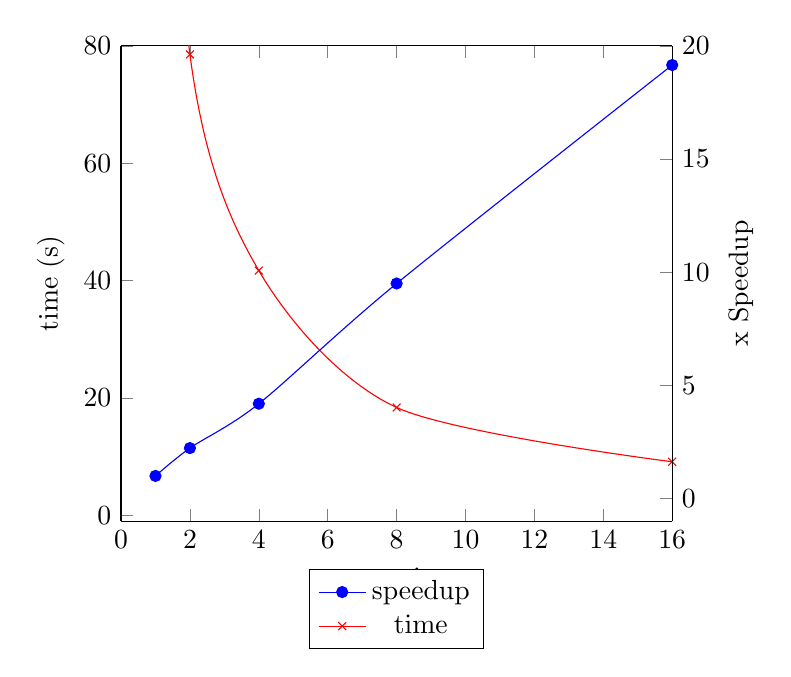
\begin{tikzpicture}
\pgfplotsset{
    scale only axis,
    %scaled x 
    xmin=0, xmax=16
}

\begin{axis}[
  axis y line*=left,
  ymin=-1, ymax=80,
  xlabel=x-axis,
  ylabel=time (s),
  legend style={at={(0.5,-0.1)},anchor=north}
]
\addplot[smooth,mark=x,red]
  coordinates{
    (1,174.83)
    (2,78.53)
    (4,41.7)
    (8,18.38)
    (16,9.13)
}; \label{plot_1}
\addlegendentry{Time}
\end{axis}

\begin{axis}[
  axis y line*=right,
  axis x line=none,
  ymin=-1, ymax=20,
  ylabel=x Speedup,
  legend style={at={(0.5,-0.1)},anchor=north}
]

% addlegendimage{/pgfplots/refstyle=plot_two}\addlegendentry{plot 2}
% APWWWSUP VALUES HERER
\addplot[smooth,mark=*,blue]
  coordinates{
    (1,1)
    (2,2.23)
    (4,4.19)
    (8,9.5)
    (16,19.15)
}; \label{plot_2} 
\addlegendentry{speedup}
\addlegendimage{smooth,mark=x,red}\addlegendentry{time}
\end{axis}
\end{tikzpicture}
\end{center}
\end{figure}

\begin{table}[H]
\centering
 \begin{tabular}{|c|c|} 
 \hline
Vertex Count & Avgerage Time (seconds)\\
 \hline
 256 &  0.70783\\ 
 \hline
 512 & 0.553\\ 
 \hline
 1024 & 4.90 \\
 \hline
 2048 & 42.6\\
 \hline
 4096 & 360.33 \\
 \hline
\end{tabular}
\caption{Results using 4 processors on the cluster}
\end{table}

\label{sec:timevert}
\begin{figure}[h]
\caption{Graph showing time and overall time per node for different node counts}
\begin{center}
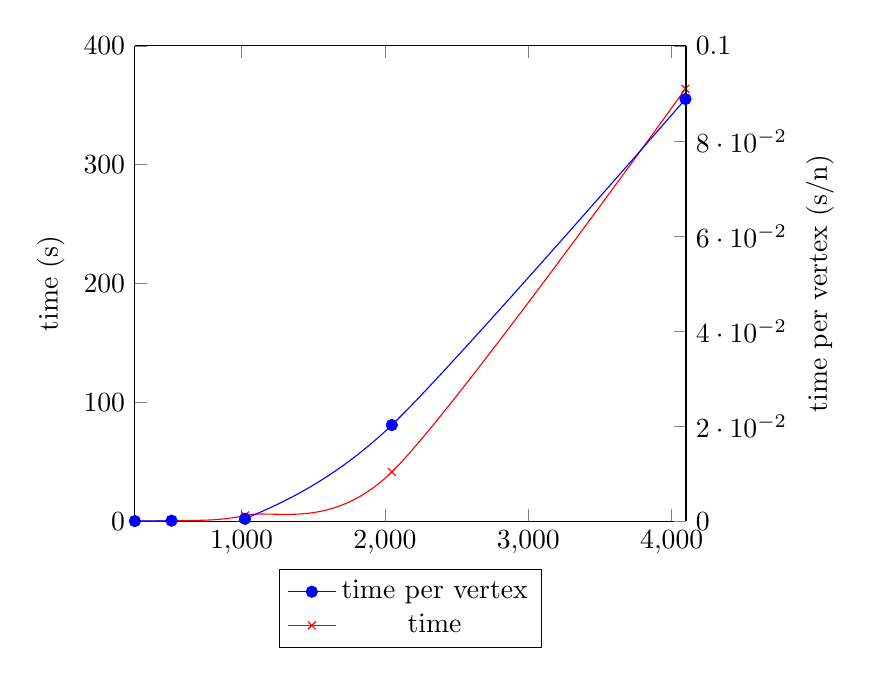
\begin{tikzpicture}
\pgfplotsset{
    scale only axis,
    %scaled x 
    xmin=256, xmax=4100
}

\begin{axis}[
  axis y line*=left,
  ymin=0, ymax=400,
  xlabel=x-axis,
  ylabel=time (s),
  legend style={at={(0.5,-0.1)},anchor=north}
]
\addplot[smooth,mark=x,red]
  coordinates{
    (256,0.070743)
    (512,0.556)
    (1024,4.8091)
    (2048,41.42)
    (4096,363.9)
}; \label{plot_1}
\addlegendentry{Time}
\end{axis}

\begin{axis}[
  axis y line*=right,
  axis x line=none,
  ymin=0, ymax=0.1,
  ylabel=time per vertex (s/n),
  legend style={at={(0.5,-0.1)},anchor=north}
]

% addlegendimage{/pgfplots/refstyle=plot_two}\addlegendentry{plot 2}
\addplot[smooth,mark=*,blue]
  coordinates{
    (256,0.0000276)
    (512,0.000108)
    (1024,0.000496)
    (2048,0.020226)
    (4096,0.0888)
}; \label{plot_2} 
\addlegendentry{time per vertex}
\addlegendimage{smooth,mark=x,red}\addlegendentry{time}
\end{axis}
\end{tikzpicture}
\end{center}
\end{figure}



\subsection{Analysis}
All tests above were tested twice. This was mainly due to limitations in access to the cluster where over 17000 jobs where scheduled to run.  

\subsection{Performance Metrics}
\subsubsection{Parallel Overhead}
Parallel overhead (\(T_o\)) is the additional execution that comes from using parallel functionality and can be calculated with:
\[T_o = pT_p + T_s\] \\
Using the varying processor count test, the average parallel overhead is \(T_o = 23.28\)s. It should be noted that this overhead affected the overall time of the smaller node counts of 256 and 512 much more as given the speed of the machines tested on the majority of the time would have been spent communicating. 
%2:  -17.77
%4:  -10.83
%8:  -27.79
%16: -28.75

\subsubsection{Speedup}
\label{speeedup}
Speedup \(S\) is the ratio of serial to parallel execution time and is calculated with:
\[S = \frac{T_s}{T_p}\] \\
Using the processor count test, the average speedup is \(S = 8.77\)
% look at change in speedup?
As seen in \ref{fig:speed}, speedup is mostly linear with an increase in processors. This indicates that the overhead of processor communication is not hindering performance under 16 processors.
\\\\
Theoretically, process speedup is limited by the amount of processors being used. However, this test provided consistent speedup greater than this bound. This could be possible under two circumstances. One possibility is that the sequential execution time is not the best implementation.
\\\\
Another possibility is that this implementation is achieving super-linear speedup. This typically occurs when hardware is exploited. A graph with 2048 vertices requires approximately 16000 kilobytes to represent as an adjacency matrix. It is possible that the sequential implementation could not fit the entire matrix into cache as efficiently, whereas the distributed implementation that distributed the matrix in smaller chunks could fit the matrix into cache more effectively.
%(ref) <https://www.bbc.co.uk/bitesize/guides/zmb9mp3/revision/3>
%2:  2.23
%4:  4.19
%8:  9.5
%16: 19.15 

\subsubsection{Efficiency}
Efficiency \(E\) is the measure of useful parallel execution time, ie. the speedup per processor. A value over 1 indicates an increase in efficiency. It can be calculated with
\[E = \frac{S}{p} = \frac{T_S}{pT_p}\] \\
Using the processor count test, the average efficiency is \(E = 1.14\), which would indicate a free performance gain simply for choosing to use the parallel algorithm. This result is highly unrealistic and could come down to a number of factors including experimental error or unusually efficient use of cache as motioned in \ref{speeedup}. Upon running more tests locally it was apparent that the larger input files were more efficient due to the increased ratio of computation time to communication although this trend would be expected to fatten out as the time spent actually transferring large amounts of data increases. 

%2:  1.12
%4:  1.05
%8:  1.19
%16: 1.20

\subsection{Time Per Vertex}
Time per vertex \(T_v\), although not specifically a performance metric, is the average extra time added per vertex. this is calculated with:
\[T_v = \frac{T_p}{n}\] \\
The average time spent per node was 0.06 seconds, but it should be noted there was an order of magnitude difference between the lower node counts like 256 and 512 and the higher ones, most likely due to the near instant computation of the shortest paths as the entirety of the graph (104 Kb in the case of the 512 node) can be stored in the L1 cache of the processor \cite{forum}. For increasing node counts the average time spent should continue to increase as more requests to higher level memory will need to be made. 
% get average


\subsection{Results Discussion}

A reoccurring theme of all the performance metric is all the results seem to be better than what would be expected. In most cases this is due to required test sizes not being large enough to sufficient consume the resources of the servers provided, which is understandable from a teaching perspective. As such hyper linear speedup, over 100\% efficiency can be expected until more higher level memory and different cache distributions are required. 

That being said, despite these issues the general trends of high performance code were still relevant in that very small problems were dominated by communication overhead and there was significant speedup for larger problems with more processors. The implementation presented in this report should continue to scale reasonable well until a single row cannot be stored in system memory in which case more aggressive partitioning of the data will have to occur. 


\section{Conclusion}

The Floyd-Warshall algorithm lends itself easily to a parallel implementation through broadcasting the intermediate node k to all processes and enjoys significant speedup on distributed systems. Partitioning the data into rows and having each processor read its own row from an input file has been shown to been quite effective and scaled well for the required test sizes. Whilst this combination of parallel file I/O and communication has been successful, other methods such as partitioning by columns or chunk partitioning may also be very effective and scale further than row partitioning. In future a more robust testing setup including larger input files, better access to cluster resources would be required to compare such techniques to avoid unseen perturbations and hyper-linear scaling through cache utilisation. 

 \bibliographystyle{unsrt}
 \bibliography{ref.bib}

 
\end{document}